\subsection{Shopify}

La scelta di adottare \emph{Shopify} come piattaforma di gestione per le operazioni di \emph{e-commerce} è stata dettata dall’esigenza di integrare il catalogo prodotti presente 
sullo \emph{store} \emph{Shopify} di \emph{Comfortzone} su un sistema \emph{client-side} (parte di un’applicazione eseguita sul dispositivo dell’utente, non sul server). In particolare, il progetto avrebbe richiesto la possibilità di esporre i prodotti dello \emph{store} 
attraverso uno \emph{storefront} personalizzabile e di consentire aggiornamenti dinamici lato server, garantendo al contempo coerenza tra i dati mostrati all’utente e quelli effettivamente 
presenti nel catalogo aziendale.

L’adozione di \emph{Shopify} avrebbe concesso di beneficiare delle sue \emph{API} flessibili, grazie alle quali si sarebbe potuto interfacciare un agente con il catalogo prodotti in tempo reale. 
Tale connessione avrebbe reso l’agente in grado di consultare, filtrare e proporre articoli in base a parametri aggiornati come prezzo, disponibilità e varianti, 
migliorando così la qualità e la pertinenza delle risposte offerte agli utenti.

Inoltre, l’integrazione con le \emph{Storefront API} (interfaccia o vetrina digitale attraverso cui un utente interagisce con un negozio online) e le \emph{Admin API} di \emph{Shopify} avrebbe reso possibile simulare le operazioni più comuni di un utente, come la 
costruzione e la gestione del carrello o la consultazione delle informazioni di prodotto, direttamente all’interno del flusso conversazionale dell’agente. Questo avrebbe consentito di 
estendere la sperimentazione anche agli aspetti di interazione e di esperienza d’acquisto, valutando l’efficacia di un approccio agentico nel guidare l’utente verso la conversione.

Infine, la scelta di \emph{Shopify} sarebbe risultata coerente con gli obiettivi del progetto anche in termini di rapidità di sviluppo e mantenibilità: 
la piattaforma avrebbe offerto strumenti di integrazione immediati, un ampio supporto documentale e una gestione semplificata del ciclo di vita dei prodotti, 
elementi ideali per la costruzione di un \emph{Proof of Concept} destinato a essere rapidamente testato e iterato.

\begin{figure}[H]
    \centering
    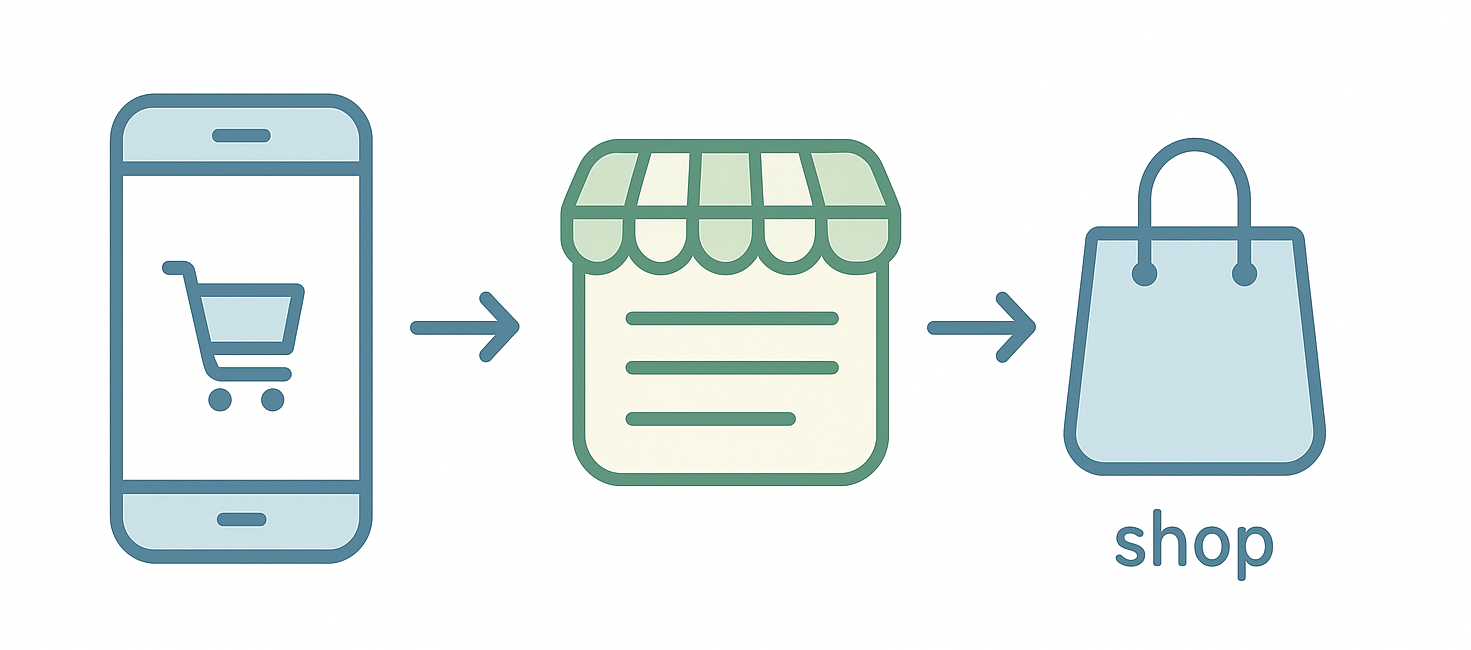
\includegraphics[width=0.8\textwidth]{stage/shopify}
    \caption{Flusso semplificato delle operazioni e-commerce tramite Shopify.}
    \label{fig:shopify}
\end{figure}